%&latex
%&latex
\documentclass[namedreferences]{SolarPhysics}
\usepackage[optionalrh,solaenum]{spr-sola-addons} % For Solar Physics 
%\usepackage{epsfig}          % For eps figures, old commands
\usepackage{graphicx}        % For eps figures, newer & more powerfull
%\usepackage{courier}         % Change the \texttt command to courier style
%\usepackage{natbib}         % For citations: redefine \cite commands
%\usepackage{amssymb}        % useful mathematical symbols
\usepackage{color}           % For color text: \color command
\usepackage{url}             % For breaking URLs easily trough lines
\def\UrlFont{\sf}            % define the fonts for the URLs


% General definitions
% please place your own definitions here and don't use \def but
% \newcommand{}{} or 
% \renewcommand{}{} if it is already defined in LaTeX

\newcommand{\BibTeX}{\textsc{Bib}\TeX}
\newcommand{\etal}{{\it et al.}}

% Definitions for equations
\newcommand{\deriv}[2]{\frac{{\mathrm d} #1}{{\mathrm d} #2}}
\newcommand{\rmd}{ {\ \mathrm d} }
\renewcommand{\vec}[1]{ {\mathbf #1} }
\newcommand{\uvec}[1]{ \hat{\mathbf #1} }
\newcommand{\pder}[2]{ \f{\partial #1}{\partial #2} }
\newcommand{\grad}{ {\bf \nabla } }
\newcommand{\curl}{ {\bf \nabla} \times}
\newcommand{\vol}{ {\mathcal V} }
\newcommand{\bndry}{ {\mathcal S} }
\newcommand{\dv}{~{\mathrm d}^3 x}
\newcommand{\da}{~{\mathrm d}^2 x}
\newcommand{\dl}{~{\mathrm d} l}
\newcommand{\dt}{~{\mathrm d}t}
\newcommand{\intv}{\int_{\vol}^{}}
\newcommand{\inta}{\int_{\bndry}^{}}
\newcommand{\avec}{ \vec A}
\newcommand{\ap}{ \vec A_p}
\newcommand{\bb}{ \vec B}
\newcommand{\jj}{ \vec j}
\newcommand{\rr}{ \vec r}
\newcommand{\xx}{ \vec x}

% Definitions for the journal names
\newcommand{\adv}{    {\it Adv. Space Res.}}
\newcommand{\annG}{   {\it Annales Geophysicae}}
\newcommand{\aap}{    {\it Astron. Astrophys.}}
\newcommand{\aaps}{   {\it Astron. Astrophys. Suppl.}}
\newcommand{\aapr}{   {\it Astron. Astrophys. Rev.}}
\newcommand{\ag}{     {\it Ann. Geophys.}}
\newcommand{\aj}{     {\it Astron. J.}}
\newcommand{\apj}{    {\it Astrophys. J.}}
\newcommand{\apss}{   {\it Astrophys. Space Sci.}}
\newcommand{\cjaa}{   {\it Chin. J. Astron. Astrophys.}}
\newcommand{\gafd}{   {\it Geophys. Astrophys. Fluid Dyn.}}
\newcommand{\grl}{    {\it Geophys. Res. Lett.}}
\newcommand{\ijga}{   {\it Int. J. Geomag. Aeron.}}
\newcommand{\jastp}{  {\it J. Atmos. Solar Terr. Phys.}}
\newcommand{\jgr}{    {\it J. Geophys. Res.}}
\newcommand{\mnras}{  {\it Mon. Not. Roy. Astron. Soc.}}
\newcommand{\nat}{    {\it Nature}}
\newcommand{\pasp}{   {\it Pub. Astron. Soc. Pac.}}
\newcommand{\pasj}{   {\it Pub. Astron. Soc. Japan}}
\newcommand{\pre}{    {\it Phys. Rev. E}}
\newcommand{\solphys}{{\it Solar Phys.}}
\newcommand{\sovast}{ {\it Sov. Astron.}}
\newcommand{\ssr}{    {\it Space Sci. Rev.}}


%%%%%%%%%%%%%%%%%%%%%%%%%%%%%%%%%%%%%%%%%%%%%%%%%%%%%%%%%%%%%%%%%%
\begin{document}

\begin{article}

\begin{opening}

\title{Article preparation guidelines\\ {\it Solar Physics}}

\author{P.~\surname{Author-a}$^{1}$\sep
        E.~\surname{Author-b}$^{1}$\sep
        M.~\surname{Author-c}$^{2}$      
       }
\runningauthor{Author-a et al.}
\runningtitle{Example paper}

   \institute{$^{1}$ First affiliation
                     email: \url{e.mail-a} email: \url{e.mail-b}\\ 
              $^{2}$ Second affiliation
                     email: \url{e.mail-c} \\
             }

\begin{abstract}
The derivation of kinematic profiles for eruptive events is prominent in the field of solar physics. The details on the acceleration of coronal mass ejections (CMEs) and large-scale coronal disturbances (`EIT waves') are important for indicating the driving mechanisms at play. The techniques used for deriving the velocity and acceleration profiles of events based upon the height-time tracks .....


\end{abstract}
\keywords{CME, EIT Waves, Corona, Mathematical Techniques}
\end{opening}
%-------------------------------------------------

\section{Introduction}
     \label{S-Introduction} 



 

\section{Numerical Differentiation Techniques} %%%%%%%%%%%%%%%%%%%%%%%%%%%%%%%%%%%%%%%%
      \label{S-general}      

\subsection{Forward/Reverse Differentiation} %%%%%%%%%%%%%%

The forward differencing technique involves the computation of the derivative at the point $t + \Delta t$ by extrapolating forward from the point $t$. This uses the Taylor series:
\begin{equation}
r(t + \Delta t) = r(t) + r'(t)\Delta t +  \frac{r''(t)}{2!}(\Delta t)^{2} + \frac{r'''(t)}{3!}(\Delta t)^{3}  + ...
\end{equation}
This equation can be re-arranged to give
\begin{equation}
r'(t)\Delta t = r(t + \Delta t) - r(t) -  \frac{r''(t)}{2!}(\Delta t)^{2} - \frac{r'''(t)}{3!}(\Delta t)^{3}  + ...
\end{equation}
which then gives
\begin{equation}
r'(t) = \frac{r(t + \Delta t) - r(t)}{\Delta t} -  \frac{r''(t)}{2!}(\Delta t) - \frac{r'''(t)}{3!}(\Delta t)^{2}  + ...
\end{equation}
This is usually written as
\begin{equation}
r'(t) = v = \frac{r(t + \Delta t) - r(t)}{\Delta t} + O(\Delta t)
\end{equation}
where $O(\Delta t)$ is the truncation error term, determined by the distance between neighbouring points ($\Delta t$). This technique assumes a straight line gradient between points. 

This estimate of the velocity is dependent on the initial units used for the distance. In the case of the simulation work done here, the units of distance are mega-metres (1~Mm = $10^6$~m). This produces an estimate of velocity in units of Mm~s$^{-1}$. To convert this to acceptable units of km~s$^{-1}$ requires multiplying the estimated velocity values by $10^{3}$. This has been done in all plots showing the numerically derived velocity. Similarly, converting the acceleration from units of Mm~s$^{-2}$ requires multiplying the estimated acceleration values by $10^{6}$.

%The forward-difference technique may be used to obtain the velocity and acceleration of the data numerically, without the use of fits. If the data can be modeled as a linear function of the form $r(t) = r_0 + v_0 t$, with a noise term of the form $\delta r$ added to the distance data (i.e.:\ $r(t) = r_0 + v_0 t + \delta r$), the velocity of the data can be estimated as
%\begin{equation}
%v = v_{0} + \frac{\delta r_{(t + \Delta t)} - \delta r_{t}}{\Delta t}
%\end{equation} 
%In this case, the velocity is estimated as the initial velocity $v_0$ with a correction term that accounts for the variation in the original data-set due to noise. This correction term is unique to each data-point due to the random nature of the applied noise.

It is possible to derive the value of the truncation error term in terms of the original $r(t)$ values. The truncation error is given as
\begin{equation}
O(\Delta t) = \frac{r''(t)}{2!}(\Delta t)
\end{equation}
The $r''(t)$ term may be decomposed using the original forward-difference definition:
\begin{equation}
r''(t) = \frac{r'(t + \Delta t) - r'(t)}{\Delta t}
\end{equation}
Rewriting each term using the original functional forms produces
\begin{equation}
O(\Delta t) = \frac{r(t + 2\Delta t) - 2r(t + \Delta t) + r(t)}{2!\Delta t}
\end{equation}
The error term associated with the velocity estimate using the forward-difference technique is therefore dependent on the value of the function $r(t)$ at the points $t$, $t+\Delta t$ and $t+2\Delta t$.

This equation must be modified when dealing with the error associated with the acceleration estimate. In this case, the truncation error term would be given as:
\begin{equation}
O(\Delta t) = \frac{v(t + 2\Delta t) - 2v(t + \Delta t) + v(t)}{2!\Delta t}
\end{equation}
Here, the velocity function $v(t)$ is treated as the base function, rather than the distance function $r(t)$ as above. 

The forward-difference technique is a very simplistic technique that produces spiky plots, with large variation between points. This is a result of the inherent assumption made by the forward-difference technique that there is a straight-line gradient between points. In addition, the forward-difference technique removes a point from the end of the data-set with each differentiation due to the way it calculates the derivative.


\subsection{Centre Differentiation}

\subsection{Lagrangian Interpolation}



    
\section{Models} %%%%%%%%%%%%%%%%%%%%%%%%%%%%%%%%%%%%%%%%
      \label{S-features}      

\subsection{const. vel.}

\subsection{const. accel.}

\subsection{non-const. accel.}

\subsection{ Cadence}

\subsection{S/N}

\section{Data}

\subsection{CMEs}

\subsection{EIT waves}

\section{Bootstrapping}

      
\subsection{Using \BibTeX} %%%%%%%%%%%%%%
  \label{S-BibTeX}
  %{\S}{\bf --- Why using \BibTeX ? } \\
  The use of \BibTeX\ simplifies the inclusion of references. Only the 
references cited and labeled in the text are included at compilation, 
and an error message appears if some references
are missing.  Any new reference will automatically be written at the correct 
location in the reference list after compilation. 
Moreover the references are stored, in any order, in a separate file
(with the \texttt{.bib} extension) in the \BibTeX\ format, so independently of 
the journal format. Such a personal reference file can be re-used with any journal.
The formatting of the references and their listing order are made automatically
at compilation (using the information given in the \texttt{.bst} file). 
        
  %{\S}{\bf --- Downloading references} \\
  The references in \BibTeX\ format can be downloaded from the 
Astrophysics Data System (ADS), then stored
in \verb+SOLA_bibliography_example.bib+  (file name of the present example).
The main extra work is to define a proper and easy label for each citation
(a convenient one is simply first-author-name-year).  Furthermore, it is better
to have the journal names defined by commands (for example 
\texttt{$\backslash$solphys)}, as defined at the beginning of 
this \texttt{.tex} file.
This provides an homogeneity in the reference list and permits flexibility
when changing for journals.   Some caution should be taken for some journals
since ADS does not necessarily provide a uniform format for the
journal names. This is the case for \jgr\  Moreover since
\jgr\ has a new way to refer to an article 
(since 2002 it has no page number), then the ADS references need to be corrected. 
More generally, it is worth verifying
each reference from the original publication (independently of \BibTeX\ use).

  %{\S}{\bf --- Compilation: general} \\
   The full \LaTeX\ and \BibTeX\ compilation is made in four steps: 
\begin{tabbing}
1) {\tt latex filename}\qquad\qquad\=(stores the labels in the {\tt .aux} file)\\
2) {\tt bibtex filename}\>(loads the bibliography in the {\tt .bbl} file)\\
3) {\tt latex filename}\>(reads the .bbl, stores in the {\tt .aux})\\
4) {\tt latex filename}\>(replaces all labels)  
\end{tabbing}
   where \texttt{filename} is the name of your \LaTeX\ file (for example, 
the present file) {\bf without} typing its \texttt{.tex} extension.
If a \texttt{(?)} is still present in the output (at the place of a label),
it means that this label has not been properly defined. 
 (for example, \LaTeX\ labels are case sensitive).
Any undefined label has a warning written in the \texttt{console window}
(it is better to have this window open by default, since \LaTeX\ warning and 
error messages are very useful to localize the problem).

  %{\S}{\bf --- Compilation: simple} \\
  When the references are not changed, it is unnecessary to re-run \BibTeX .
When no new labels are added, running latex once is sufficient to refresh
the \LaTeX\ output. So, except for
the first, and the final time (safest), running \LaTeX\ once is sufficient
in most cases to update the \LaTeX\ output, if the compilation files 
created are not erased! For example \BibTeX\ keeps the bibliography in the usual 
environment,\\
  \verb+ \begin{thebibliography}{} ... \end{thebibliography}+\\
in the file with the \verb+.bbl+ extension.  

\subsection{Miscellaneous Other Features} %%%%%%%%%%%%%%
      \label{S-Miscellaneous} 
Long URL's can be quite messy when broken across lines
\texttt{ http://gong.nso.edu/data/magmap/} as normal text,
however the \texttt{url} package does a nice job of this, \textit{e.g.} 
\url{http://gong.nso.edu/data/magmap/}.
   
\section{Conclusion} %%%%%%%%%%%%%%%%%%%%%%%%%%%%%%%%%%%%%%%%
      \label{S-Conclusion} 
      We hope authors of {\it Solar Physics} will find this guide useful.
Please send us feedback on how to improve it.
      
  \LaTeX\ is very convenient to write a scientific text, in particular
with the use of labels for figures, tables, and references. Moreover, the labels and list of references are checked by the software against
one another, and, the formatting should be effortless with \BibTeX.

%%%%%%%%%%%%%%%%%%%%%%%%%%%%%%%%%%%%%%%%%%%%%%%%%%%%%%%%%%%%%%%%%%%%%%%%%%%
\appendix   

 After the \verb+\appendix+ command, the sections are referenced with 
capital letters. 
The numbering of equations, figures and labels is 
is just the same as with classical sections.

  \begin{figure}    %%%%%%%%%%%%%%%%%% FIGURE 1 
   \centerline{\includegraphics[width=0.3\textwidth,clip=]{fig1a.eps}
              }
   \caption{Example of a simple figure in an appendix.}
    \label{F-appendix}
  \end{figure}

  \begin{table}
   \caption{ A simple table in an appendix. }
   \label{T-appendix}
    \begin{tabular}{ccclc}     % define the column alignment
                               % l: left, c: center, r: right
      \hline                   % horizontal line
    Rot. & Date & CMEs & CMEs~ & $\alpha$ \\
         &      & obs. & ~cor. & $10^{-2}$Mm$^{-1}$\\
      \hline
    1 & 02--Nov--97 & 16  & 24.1  & -1.26 \\
    2 & 29--Nov--97 & --  & ~2.53 & ~0.94 \\
      \hline
    \end{tabular}
   \end{table}


\section{Abbreviations of some Journal Names} %%%%%%%%%
    \label{S-appendix}
Journal names are abbreviated in {\it Solar Physics} with the IAU
convention (IAU Style Book
published in Transactions of the IAU XXB, 1988, pp. Si-S3.
\url{www.iau.org/Abbreviations.235.0.html}).  Here are a few journals with their \LaTeX\ 
commands (see the beginning of this \texttt{.tex} file).\\
  \verb+\aap     + \aap \\
  \verb+\apj     + \apj \\
  \verb+\jgr     + \jgr \\
  \verb+\mnras   + \mnras \\
  \verb+\pasj    + \pasj \\
  \verb+\pasp    + \pasp \\
  \verb+\solphys +~ \solphys 
  
%%%%%%%%%%%%%%%%%%%%%%%%%%%%%%%%%%%%%%%%%%%%%%%%%%%%%%%%%%%%%%%%%%%%%%%%%%%
\begin{acks}
 The authors thank ... ({\it note the reduced point size})
\end{acks}


%%% BIBLIOGRAPHY %%%%%%%%%%%%%%%%%%%%%%%%%%%%%%%%%%%%%%%%%%%%%%%%%%%%%%%%%%%
\mbox{}~\\ 
\noindent {\normalsize \bf Bibliography Included with \BibTeX }\\* 
      % more powerful
  With \BibTeX\ the formatting will be done automatically for all 
the references cited with one
of the \verb+\cite+ commands (Section~\ref{S-references}).
Besides the usual items, it includes the title of the article 
and the concluding page number. 
   
     % format of references provided by the journal (.bst)
\bibliographystyle{spr-mp-sola}
%\bibliographystyle{spr-mp-sola-cnd} %% Alternative style: no title,
                                      % no concluding page. 

     % name your Bibtex file containing your references (.bib)
\bibliography{SOLA_bibliography_example}  

     % Checking: look if the file containing the ``\bibitem'' exits
     %           so check if the .bbl file exist (bibTeX compilation)
\IfFileExists{\jobname.bbl}{} {\typeout{}
\typeout{****************************************************}
\typeout{****************************************************}
\typeout{** Please run "bibtex \jobname" to obtain} \typeout{**
the bibliography and then re-run LaTeX} \typeout{** twice to fix
the references !}
\typeout{****************************************************}
\typeout{****************************************************}
\typeout{}}

\noindent {\normalsize \bf Bibliography included manually }\\*
     % Require more work
  The articles can be entered, formatted, and ordered  
by the author with the command \verb+\bibitem+.  ADS provides
references in the {\it Solar Physics} format by selecting
the format \verb+SoPh format+ under the menu 
\verb+Select short list format+.    Including the article title
and the concluding page number are optional;
however, we require consistency in the author's choice.
That is, all of the references should have the article title, or none,
and similarly for ending page numbers.

\begin{thebibliography}{}
  \bibitem[\protect\citeauthoryear{{Berger}}{2003}]{Berger03b}
Berger,~M.A.: 
2003, in Ferriz-Mas, A., N{\'u}{\~n}ez, M. (eds.),
    \textit{Advances in Nonlinear Dynamics}, Taylor and Francis Group, 
    London, 345.
  \bibitem[\protect\citeauthoryear{{Berger} and {Field}}{1984}]{BergerF84b}
Berger,~M.A., Field,~G.B.: 
1984, \textit{J. Fluid. Mech.} \textbf{147}, 133.
  \bibitem[\protect\citeauthoryear{{Brown}, {Canfield}, and
                                   {Pevtsov}}{1999}]{Brown99b}
Brown,~M., Canfield,~R., Pevtsov,~A.:
1999, Magnetic Helicity in Space and Laboratory Plasmas, Geophys. Mon. 
      Ser. 111, AGU.
 \bibitem[\protect\citeauthoryear{{Dupont}, {Schmidt}, and {Koutny}}{2007}]{Dupont07b}
Dupont, J.-C., Schmidt, F., Koutny, P.: 2007, \solphys{} \textbf{323}, 965. 
\end{thebibliography}

\end{article} 

\end{document}
